\documentclass[11pt]{article}
\usepackage{enumerate}
\usepackage{fancyhdr}
\usepackage{amsmath}
\usepackage{graphicx}

\thispagestyle{empty}
\setlength{\parindent}{0cm}
\setlength{\parskip}{0.3cm plus4mm minus3mm}
\oddsidemargin = 0.0in
\textwidth = 6.5 in
\textheight = 9 in
\headsep = 0in

\title{CSCI 4100 Fall 2018 \\
Assignment 2 Answers}
\author{Damin Xu\\661679187}



\begin{document}
\maketitle

\noindent{\bf Exercise 1.8}
\[
P[\nu\leq0.1]=0.1^{10}+C^{10}_1\times0.1^9\times\mu=0.1^{10}+C^1_{10}\times0.1^9\times0.9\leq9.1\times10^{-9}
\]
\\\\
\noindent{\bf Exercise 1.9}
\\Using Hoeffding Inequality: 
\[
P[|\mu-\nu|>\epsilon]\leq2e^{-2\epsilon^2N}
\]
Then:
\[
P[\nu\leq0.1]=P[|0.9-\nu|\geq0.8]
\]
Here $\mu$ = 0.9 and $\epsilon$ = 0.8, and because $N$ = 10
\[
P[|0.9-\nu|\geq0.8] \leq 2e^{-2\times0.8^2\times10} \leq 5.22\times10^{-6}
\]
By using Hoeffding Inequality, the upper bound of probability is much larger than the upper bound calculated using binominal distribution.

\newpage

\noindent{\bf Exercise 1.10}
\begin{enumerate}  [(a)]
\item $\mu$ is 0.5 since the 3 coins are fair.

\item \  
\begin{figure}[htb]        
\center{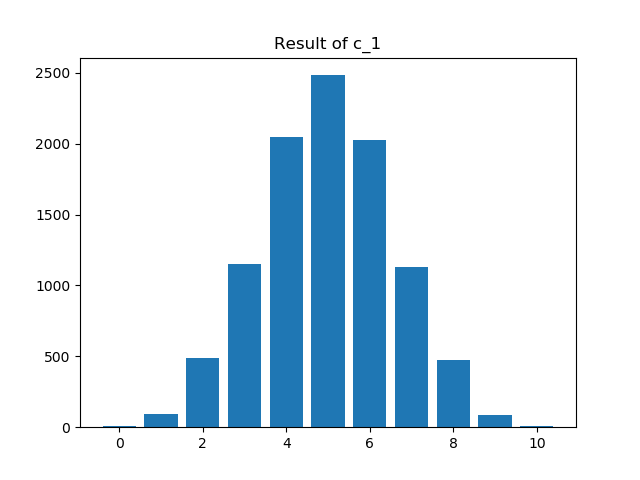
\includegraphics[height=8cm]{1_10_1.png}}        
\center{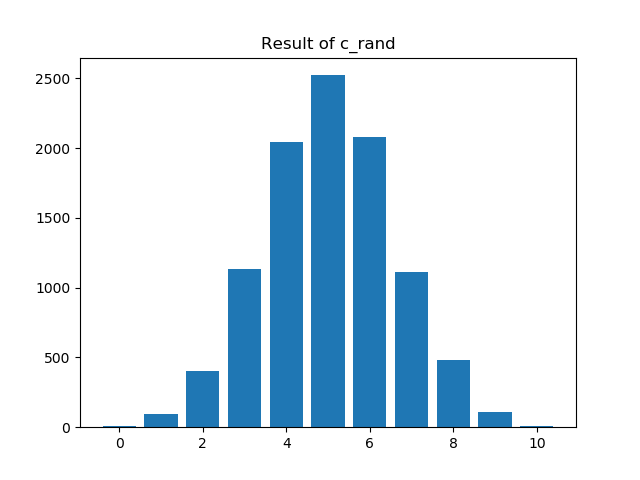
\includegraphics[height=8cm]{1_10_2.png}}
\end{figure}
\newpage
\begin{figure}[htb]        
\center{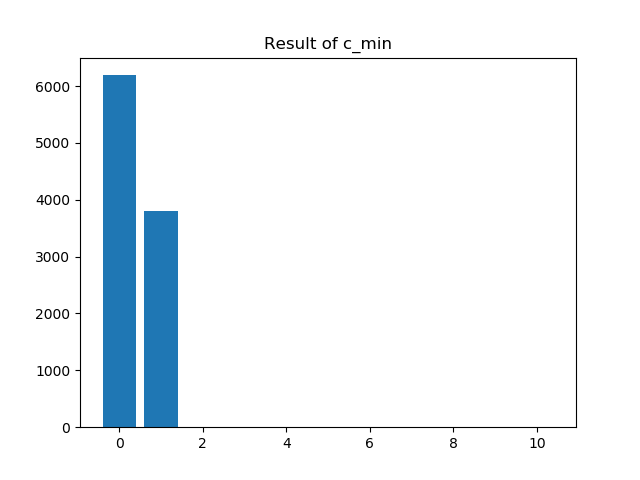
\includegraphics[height=8cm]{1_10_3.png}}        
\end{figure}

\item \
\begin{figure}[htb]        
\center{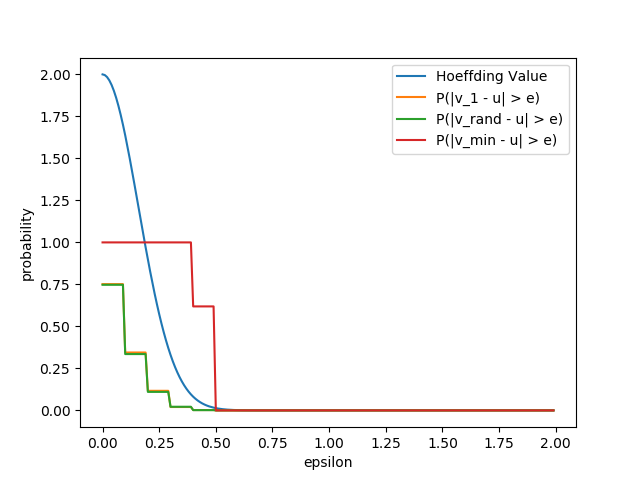
\includegraphics[height=8cm]{1_10_4.png}}        
\end{figure}

\item According to the graph in part (c), coin $c_1$ and $c_{rand}$ obey the Hoeffding bound because they decrease with Hoeffding Value decreases, but coin $c_{min}$ does not, because there is a sudden drop on graph where the Hoeffding value decreases smoothly.

\item The coin $c_{min}$ is not a sample ramdonly chosen from the bottle. We cannot choose coin with specific property, and such coin does not obey the Hoeffding bound.

\end{enumerate}

\newpage
\noindent{\bf Exercise 1.11}
\begin{enumerate} [(a)]
\item No, because using algorithm $S$ only means it works well on the given training example set $D$, but the performance outside $D$ is unsure.

\item Yes, because performances of algorithm $S$ and $C$ is alway unsure outside the traing example set $D$ whatever how they perform with $D$.

\item $p$ = 0.9, so $P(f_S=f)$ = $p$ = 0.9 and $P(f_S=f)$ = $p$ = 0.1.\\
Then:
\[
P[P(f_S=f)>P(f_S=f)]=P[0.9>0.1] = 1
\]

\item The probability that $C$ will produce better hypothesis than $S$ is that $P[P(f_S=f)>P(f_S=f)]>0.5$. To achieve this, $p$ should be smaller than 0.5 because $P[P(f_S=f)>P(f_S=f)]=P(p>1-p)$, and when $p<0.5$, $P(p>1-p)=0$
\end{enumerate}

\noindent{\bf Exercise 1.12}\\
I would like to choose $(c)$, because no one can promise the learning process can give a good hypothesis

\noindent{\bf Problem 1.3}
\begin{enumerate} [(a)]
\item Because $y_n=sign(w^{*T}x_n)$, $y_n(w^{*T}x_n)=[sign(w^{*T}x_n)]w^{*T}x_n$.\\
Thus when $w^{*T}x_n > 0$, $y_n>0$ and when $w^{*T}x_n < 0$, $y_n<0$.
So $y_n(w^{*T}x_n)$ is positive for $1\leq n\leq N$ since $N$ is limited.

\item First show that $w^T(t)w^*\geq w^T(t-1)w^*+\rho$:
LHS: according to rule 1.3 on page 7\[
\begin{aligned}
w^T(t)w^* &= [w^T(t-1)+y(t-1)x_{t}] \times w^*\\
&=w^T(t-1)w^*+y(t-1)w^{*T}x_{t-1}
\end{aligned}
\]
RHS:
\[
\begin{aligned}
w^T(t-1)w^*+\rho = w^T(t-1)w^*+ min_{1\leq n \leq N}y(t-1)w^{*T}x_{t-1}
\end{aligned}
\]
There is no doubt the LHS $\geq$ RHS.
\\\\Then, Prove $w^T(t)w^*\geq t\rho$:\\
Prove by induction:\\
Base case: when t = 0, $w^T(t)w^* = 0$ and $t\rho=0$, so $w^T(0)w^*\geq 0\rho$ is true.\\
Assume for any P(t): $t\geq 0, w^T(t)w^*\geq t\rho$ is true\\
Show that P(t+1): $w^T(t+1)w^*\geq (t+1)\rho$:\\
$RHS=(t+1)\rho = t\rho +\rho$\\
And according to the first part, $LHSw^T(t+1)w^*=w^T(t)w^*+\rho$\\
The assumption states that $w^T(t)w^*\geq t\rho$, so P(t+1) is true\\
By induction, $w^T(t)w^*\geq t\rho$.

\newpage
\item According to the part (b):\[
\begin{aligned}
LHS &= ||w(t-1)+y(t-1)x(t-1)||^2\\
	&= ||w(t-1)||^2+||y(t-1)x(t-1)||^2+2y(t-1)w^T(t-1)x(t-1)\\
	&\leq ||w(t-1)||^2+||y(t-1)x(t-1)||^2\\
	&\leq RHS,\ because\ of\ the\ hint.
\end{aligned}
\]


\item Prove by induction:\\
Base Case: P(1):\[
||w(1)||^2 \leq ||w(0)||^2+||x(0)||^2 \leq R^2
\]
Assume P(t): $||w(t)||^2 \leq tR^2$ is true,\\
Show that P(t+1): $||w(t+1)||^2 \leq (t+1)R^2$ is also true:\\
LHS: according to part (c):\[
||w(t)||^2\leq ||w(t+1)||^2+||x(t)||^2 
\]
Then due to assumption P(1), $||w(t+1)||^2 < tR^2$ and $||x(t)||^2$<R:
\[
LHS \leq tR^2+R^2 = RHS
\]
By induction, P(t+1) is true, and the assumption $||w(t)||^2 \leq tR^2$ is true. 

\item According part (b), $w^T(t)w^*\geq t\rho$.\\
According part (d), $||w(t)||^2\leq tR^2$, so $||w(t)||\leq \sqrt{t}R$
Therefore, \[
\frac{w^T(t)w^*}{||w(t)||} \geq \frac{t\rho}{\sqrt{t}R}=\frac{\sqrt{t}\rho}{R}=RHS
\]
\\
Show that $t\leq\frac{R^2||w^*||^2}{\rho^2}$:\\
According to the Cauthy-Schwarz Inequity,
\[
w^T(t)\leq||w(t)||\cdot||w^*||
\]
So,
\[
\sqrt{t}\frac{\rho}{R}\leq||w^*||
\]

\[
t\leq\frac{||w^*||^2R^2}{\rho^2}
\]
\end{enumerate}
\newpage
\noindent{\bf Problem 1.7}
\begin{enumerate} [(a)]
\item If $\mu=0.05$:\\
$P[1\ coin]=(1-0.05)^{10}=0.599$\\
$P[1000\ coin]=1-[1-(1-0.05)^{10}]^{1000}=1$\\
$P[1000000\ coin]=1-[1-(1-0.05)^{10}]^{1000000}=1$
\\\\
If $\mu=0.8$:\\
$P[1\ coin]=(1-0.8)^{10}=1.024\times10^{-7}$\\
$P[1000\ coin]=1-[1-(1-0.8)^{10}]^{1000}=1.024\times10^{-4}$\\
$P[1000000\ coin]=1-[1-(1-0.8)^{10}]^{1000000}=0.0973$

\item \ \\\begin{figure}[htb]        
\center{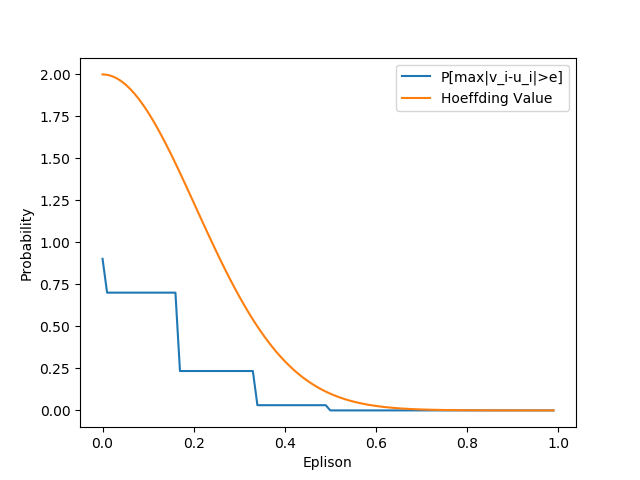
\includegraphics[height=8cm]{p_1_7.png}}        
\end{figure}


\end{enumerate}

\end{document}
\end{document}
